\documentclass{article}
\usepackage[utf8]{inputenc}
\usepackage{amsmath}
\usepackage{amssymb}
\usepackage{indentfirst}
\usepackage{graphicx}
\usepackage[a4paper, margin=1in]{geometry}
\usepackage[margin=3cm]{caption}

\usepackage{xcolor,sectsty}
\definecolor{astral}{RGB}{46,116,181}
\subsectionfont{\color{astral}}
\sectionfont{\color{astral}}


\linespread{1.15}
\title{
\includegraphics[width=0.1\textwidth]{ufallogo.png} \\\Huge{\color{astral}\textbf{Formalismo Lagrangeano da Mecânica Clássica}}}
\author{Paulo Brandão}
\date{Maio de 2017}

\begin{document}

\maketitle

\section{Introdução e Objetivos}

Existe uma grande variedade de problemas descritos pela mecânica Newtoniana onde precisamos utilizar coordenadas que não são cartesianas. Infelizmente, as expressões matemáticas das componentes da aceleração em coordenadas que não são cartesianas são bastante complicadas. Isso faz com que a segunda lei de Newton seja muito difícil de ser aplicada. Precisamos de equações do movimento alternativas (porém, equivalentes) que funcionem da mesma maneira em qualquer sistema de coordenadas. Essa alternativa é fornecida pelas equações de Lagrange, tema principal da nossa aula. A melhor maneira de provar as equações de Lagrange é utilizando um \textit{princípio variacional}. Princípios variacionais são importantes em muitas áreas da física e da matemática. Provou-se ser possível reformular quase todas as áreas da física - mecânica clássica, mecânica quântica, óptica, eletromagnetismo - em termos variacionais. Iremos introduzir métodos variacionais inicialmente num contexto geral e, após a discussão do método e sua aplicação em um problema simples, formularemos a mecânica clássica utilizando esse novo método.

\section{Funções e Funcionais}

Antes de discutir as ideias por trás do método variacional, é útil relembrar, de forma elementar, o significado de função. Uma função $f$ é uma \textit{instrução} que associa um elemento de um conjunto $A$ a um elemento de outro conjunto $B$. Indicamos essa ação como $f: A \rightarrow B$. Em geral, utiliza-se a notação $f(x)$ para indicar que a função $f$ atua em um elemento $x$ do conjunto $A$ gerando um elemento $f(x)$ do conjunto $B$. O comportamento de uma função depende exclusivamente da natureza dos conjuntos $A$ e $B$. Exemplos de funções são:
\begin{equation}
    f:\mathbb{R}\rightarrow\mathbb{R}\hspace{1cm} \text{tal que} \hspace{1cm} f(x) = x^2 \\
\end{equation}
\begin{equation}
    f:\mathbb{R}\rightarrow\mathbb{C}\hspace{1cm} \text{tal que} \hspace{1cm} f(x) = \sqrt{x^2-1}, \\
\end{equation}
onde $\mathbb{R}$ e $\mathbb{C}$ representam os conjuntos dos números reais e complexos, respectivamente. Assim, uma função tem como entrada um \textit{número} e como saída \textit{outro número}. Uma máquina de refrigerante tem como entrada uma nota de 5 reais e como saída uma lata de refrigerante. Uma função funciona como uma caixa preta onde números entram e números saem, regidos por uma instrução $f$.

Existe uma outra entidade matemática um pouco mais complicada do que uma função. Essa outra operação exótica tem como entrada, em sua caixa preta, não um número mas uma própria função. O \textit{funcional} também é um tipo de instrução que associa uma função de um conjunto $L$ a um \textit{número} no conjunto dos reais $\mathbb{R}$. Na notação discutida acima, teríamos $F:L\rightarrow\mathbb{R}$ onde $L$ é um conjunto formado por determinadas funções. Exemplos de funcionais são:
\begin{equation}
    F:L\rightarrow\mathbb{R}\hspace{1cm} \text{tal que} \hspace{1cm} F[f(x)] = \int_{0}^{1}f(x)dx
\end{equation}
\begin{equation}
    F:L\rightarrow\mathbb{R}\hspace{1cm} \text{tal que} \hspace{1cm} F[f(x)] = \int_{x_1}^{x_2}\sqrt{1+\left[\frac{df(x)}{dx}\right]^2}dx. 
\end{equation}
Note que 
\begin{equation}
    F:L\rightarrow\mathbb{R}\hspace{1cm} \text{tal que} \hspace{1cm} F[f(x)] = \sqrt{1+\left[\frac{df(x)}{dx}\right]^2}dx. 
\end{equation}
\textbf{não} é um funcional, pois não retorna um número.

Você pode pensar que esses seres mais exóticos da matemática não desempenham um papel no mundo físico. Porém, vários problemas de origem física e matemática são governados por funcionais. Para demonstrar apenas um desses problemas, considere o seguinte: Suponha que no plano $(x,y)$ estejam marcados dois pontos, 1 e 2, com coordenadas $(x_1,y_1)$ e $(x_2,y_2)$. Podemos inventar um número infinitos de funções $y(x)$ que ligam esses dois pontos no plano. O único pré-requisito que essas funções precisam cumprir é que $y(x_1) = y_1$ e $y(x_2)=y_2$. A pergunta que queremos responder é: Dada uma função $y(x)$, qual seu comprimento? Um elemento infinitesimal de comprimento, $ds$, de qualquer curva arbitrária que liga os dois pontos é dado por
\begin{equation}
    ds = \sqrt{dx^2+dy^2} = \sqrt{1+\left( \frac{dy}{dx} \right)^{2}}dx,
\end{equation}
de modo que o comprimento total da curva é 
\begin{equation}
    S = \int ds = \int_{x_1}^{x_2}\sqrt{1+\left( \frac{dy}{dx} \right)^{2}}dx = S[y(x)].
\end{equation}
Note que $S$ é um funcional (de fato, ele apareceu nos exemplos anteriores) e dada uma função $y(x)$ ele retorna o comprimento total da curva. Para tornar o problema ainda mais interessante, podemos perguntar qual função, das infinitas funções $y(x)$ existentes, possui o menor comprimento? Esse problema parece ser bastante complicado e, para piorar, observe que a função $y(x)$ está dentro da integral! Como podemos encontrar a função $y(x)$ que faz com que $S$ tenha um valor mínimo? O que esse problema tem a ver com a mecânica clássica? Iremos responder essas perguntas na próxima seção.

\section{Princípio de Hamilton}

Dois tipos fundamentais de energia aparecem na descrição do movimento de uma partícula. A energia cinética, $K$, associada ao movimento da massa, e a energia potencial, $U$, associada às forças conservativas que atuam no objeto. Uma quantidade extremamente útil, é a energia total, $E_T$ dada pela soma das duas energias $K+U$. Existe uma outra quantidade muito útil no estudo da mecânica que pode ser definida como a \textit{diferença} entre $K$ e $U$ chamada de \textbf{Lagrangeano},
\begin{equation}
    L(\mathbf{r},\dot{\mathbf{r}}) = \frac{1}{2}m\dot{\mathbf{r}}\cdot\dot{\mathbf{r}} - U(\mathbf{r}),
\end{equation}
onde utilizei a notação $\dot{\mathbf{r}} = d\mathbf{r}/dt$. Observe mais uma vez o sinal de menos utilizado na definição do Lagrangeano que não representa, portanto, a energia total do sistema. O método variacional aparece na mecânica por conta do 

\vspace{0.5cm}

\noindent\textit{PRINCÍPIO DE HAMILTON}: A trajetória real de uma partícula que se move entre dois pontos 1 e 2 num dado intervalo de tempo, de $t_1$ até $t_2$, é tal que a integral de ação $S = \int_{t_1}^{t_2}Ldt$ é estacionária, quando calculada ao longo da trajetória real. 

\vspace{0.5cm}

\noindent Com  ``trajetória real'' queremos dizer a trajetória no mundo real, isto é, a trajetória física que a partícula realmente irá descrever no espaço dadas as circunstânceas do problema. O significado de estacionário aqui é que o valor de $S$ pode ser um máximo, um mínimo ou um ponto de inflexão. Perceba que temos agora um problema variacional onde a solução que queremos encontrar, a posição da partícula $\mathbf{r}(t)$, se encontra dentro de uma integral. A ação $S$ é, portanto, um funcional, como descrito na seção anterior.

Estamos preparados agora para demonstrar que as equações do movimento de Newton aparecem como uma consequência do princípio de Hamilton. Para simplificar um pouco, iremos assumir que o movimento ocorre apenas em uma direção, por exemplo, a partícula se move apenas no eixo $x$. O caso geral é facilmente generalizado. Assim, o Lagrangeano depende explicitamente apenas da variável $x$ e de sua derivada: $L(x,\dot{x})$. O princípio de Hamilton diz que 
\begin{equation}
    S = \int_{t_1}^{t_2}L(x,\dot{x})dt
\end{equation}
é estacionária quando $x(t)$ é a trajetória real seguida pela partícula. Podemos criar trajetórias ligeiramente diferentes se escrevermos $X(t) = x(t) + \alpha\epsilon(t)$ onde $\alpha$ é uma constante real e $\epsilon(t)$ um desvio da trajetória. Assumindo que os pontos inicial e final são fixos, isto é, $\epsilon(t_1) = \epsilon(t_2) = 0$, teremos
\begin{equation}
    S(\alpha) = \int_{t_1}^{t_2}L(X,\dot{X})dt,
\end{equation}
e a condição estacionária pode ser escrita como
\begin{equation}
\frac{dS(\alpha)}{d\alpha}\Bigr|_{\substack{\alpha=0}} = \int_{t_1}^{t_2}\frac{\partial L}{\partial\alpha}\Bigr|_{\substack{\alpha=0}}dt.
\end{equation}
Vamos tratar o integrando separadamente para facilitar a visualização dos cálculos. Explicitamente temos:
\begin{equation}
\begin{split}
    \frac{\partial L}{\partial\alpha}\Bigr|_{\substack{\alpha=0}} & = \left( \frac{\partial L}{\partial X}\frac{\partial X}{\partial\alpha} + \frac{\partial L}{\partial \dot{X}}\frac{\partial \dot{X}}{\partial\alpha} \right)\Bigr|_{\substack{\alpha=0}} \\
    & = \left( \frac{\partial L}{\partial X}\epsilon(t) + \frac{\partial L}{\partial \dot{X}}\dot{\epsilon}(t) \right)\Bigr|_{\substack{\alpha=0}} \\
    & = \frac{\partial L}{\partial x}\epsilon(t) + \frac{\partial L}{\partial \dot{x}}\dot{\epsilon}(t),
    \end{split}
\end{equation}
note que na última linha utilizei a condição $\alpha = 0$, que implica $X(t) = x(t)$. Substituindo de volta na equação (11):
\begin{equation}
\frac{dS(\alpha)}{d\alpha}\Bigr|_{\substack{\alpha=0}} = \int_{t_1}^{t_2}\left[\frac{\partial L}{\partial x}\epsilon(t) + \frac{\partial L}{\partial \dot{x}}\dot{\epsilon}(t)\right]dt.
\end{equation}
Para colocar a integral numa forma mais clara, vamos utilizar a igualdade
\begin{equation}
    \int \dot{u}vdt = [uv] - \int u\dot{v}dt
\end{equation}
no segundo termo do integrando da equação (13), com $\dot{u}= \dot{\epsilon}$ e $v = \partial L/\partial \dot{x}$:
\begin{equation}
    \int_{t_1}^{t_2}\frac{\partial L}{\partial \dot{x}}\dot{\epsilon}(t)dt = -\int_{t_1}^{t_2} \epsilon(t)\frac{d}{dt}\frac{\partial L}{\partial \dot{x}}dt
\end{equation}
onde o termo de contorno é nulo pois $\epsilon(t_1) = \epsilon(t_2) = 0$ (os pontos inicial e final são fixos). Juntando tudo, temos a seguinte relação
\begin{equation}
    \frac{dS(\alpha)}{d\alpha}\Bigr|_{\substack{\alpha=0}} = \int_{t_1}^{t_2}\epsilon(t)\left[\frac{\partial L}{\partial x}-\frac{d}{dt}\frac{\partial L}{\partial \dot{x}}\right]dt = 0,
\end{equation}
que é satisfeita caso o integrando que multiplica $\epsilon(t)$ (que é uma função arbitrária diferente de zero) seja nulo. Assim derivamos as chamadas Equações de Euler-Lagrange:
\begin{equation}
    \frac{\partial L}{\partial x}-\frac{d}{dt}\frac{\partial L}{\partial \dot{x}} = 0.
\end{equation}
Portanto, a trajetória de uma partícula, $x(t)$, será aquela descrita por uma Lagrangeana que satisfaz a equação de Euler-Lagrange acima. Para mostrar a equivalência entre a equação (17) e a segunda lei de Newton, vamos substituir na relação (17) o Lagrangeano da partícula em uma dimensão: 
\begin{equation}
    L(x,\dot{x}) = \frac{m\dot{x}^2}{2} - U(x),
\end{equation}
o resultado é
\begin{equation}
    -\frac{dU(x)}{dx} - m\ddot{x} = 0,
\end{equation}
como $F_{x} = -dU(x)/dx$ é a força na direção $x$, temos que $F_{x} = ma_{x}$, onde $a_x = \ddot{x}$, que é a segunda lei de Newton. A generalização para três coordenadas espaciais, $(x,y,z)$, é facilmente obtida e será proposta como um exercício para os alunos. O resultado que o aluno deve demonstrar é que, se o Lagrangeano for da forma $L(x,y,z,\dot{x},\dot{y},\dot{z})$, cada coordenada irá separadamente satisfazer uma equação de Euler-Lagrange:
\begin{equation}
        \frac{\partial L}{\partial x}-\frac{d}{dt}\frac{\partial L}{\partial \dot{x}} = 0,
\end{equation}
\begin{equation}
        \frac{\partial L}{\partial y}-\frac{d}{dt}\frac{\partial L}{\partial \dot{y}} = 0,
\end{equation}
\begin{equation}
        \frac{\partial L}{\partial z}-\frac{d}{dt}\frac{\partial L}{\partial \dot{z}} = 0.
\end{equation}

\section{Coordenadas Generalizadas}

Mostramos na seção anterior como a segunda lei de Newton pode ser reformulada em termos da função Lagrangeana do sistema, porém não ficou claro de que forma podemos utilizar essa função na solução de problemas práticos. Um outro ponto importante é que utilizamos na derivação das equações de Euler-Lagrange um sistema de coordenadas cartesianas e, como foi comentado no início dessa aula, nem sempre coordenadas cartesianas são úteis na solução de problemas. Iremos primeiramente generalizar as equações de Euler-Lagrange para qualquer tipo de coordenada, chamadas \textbf{coordenadas generalizadas}.

Considere um sistema arbitrário de $N$ partículas, $\alpha = 1,...,N$ com posições $\mathbf{r}_{\alpha}$. Dizemos que os parâmetros $q_1,...,q_n$ formam um conjunto de \textbf{coordenadas generalizadas} para o sistema se cada posição $\mathbf{r}_\alpha$ pode ser escrita como função de $q_1,...,q_N$, e possivelmente do tempo $t$,
\begin{equation}
    \mathbf{r}_\alpha = \mathbf{r}_\alpha(q_1,...,q_N,t)\hspace{1cm}[\alpha = 1,...,N],
\end{equation}
e, da mesma forma, cada $q_i$ pode ser escrito em termos de $\mathbf{r}_\alpha$ e possivelmente do tempo $t$,
\begin{equation}
    q_i = q_i(\mathbf{r}_1,...,\mathbf{r}_N,t)\hspace{1cm}[i = 1,...,n].
\end{equation}
Além dessas condicões, para que os parâmetros $q_1,...,q_n$ formem um conjunto de coordenadas generalizadas, exigimos que \textbf{o número de coordenadas generalizadas} ($n$) \textbf{seja o menor número possível capaz de caracterizar o sistema}. Os três exemplos a seguir ilustram o uso das relações (23) e (24).

\subsubsection*{Ex. 1: O Pêndulo Simples no Plano ($N = 1$ e $n = 1$)}

Para descrever completamente o sistema, precisamos da posição $x$ e $y$ da massa presa ao pêndulo (assumindo que ele se move em duas dimensões). No entanto, podemos igualmente descrever a massa da partícula através de um único número $\theta$ (que não possui dimensão de comprimento). O valor de $\theta$ é o ângulo entre a vertical e o fio na qual a massa está presa (veja a figura abaixo). A coordenada generalizada do sistema é $q_1 = \phi$ e, através da figura, podemos escrever $\mathbf{r}=(x,y)  = (l\sin\phi,l\cos\phi)$. Dessa forma temos $x = x(\phi)$, $y = y(\phi)$ e $\phi = \phi(x,y)$.

\begin{figure}[h]
\centering
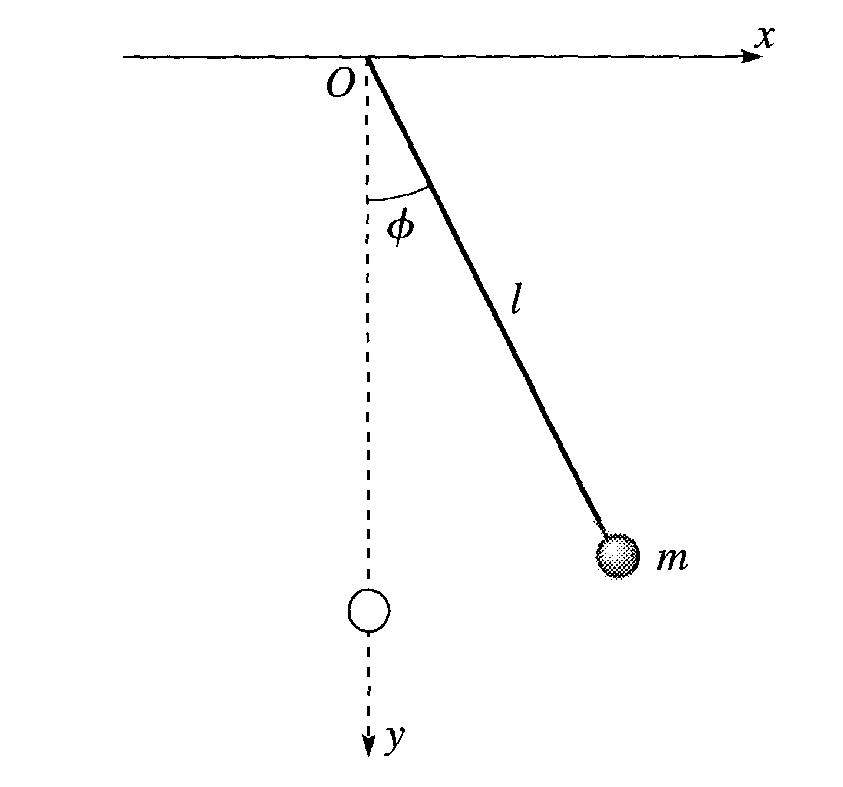
\includegraphics[width=4cm]{pendulum.png}
\end{figure}

\subsubsection*{Ex. 2: O Pêndulo Duplo no Plano ($N = 2$ e $n=2$)}

Para descrever completamente o sistema, precisamos das posições $x_1$ e $y_1$ da massa 1 presa ao ponto de apoio e das posições $x_2$ e $y_2$ da massa 2 presa à massa 1. Ou seja, precisamos de quatro números $(x_1,y_1,x_2,y_2)$. No entanto, podemos igualmente descrever o sistema através dois parâmetros $\theta_1$ e $\theta_2$ (que não possuem dimensão de comprimento, veja a figura abaixo). Assim, é possível reduzir a quantidade de coordenadas necessárias para caracterizar o sistema. Neste caso, temos 
\begin{equation}
    \mathbf{r}_1 = (l_1\sin\phi_1,l_1\cos\phi_1) = \mathbf{r}_1(\phi_1)
\end{equation}
\begin{equation}
    \mathbf{r}_2 = (l_1\sin\phi_1 + l_2\sin\phi_2,l_1\cos\phi_1+l_2\cos\phi_2) = \mathbf{r}_2(\phi_1,\phi_2)
\end{equation}

\begin{figure}[h]
\centering
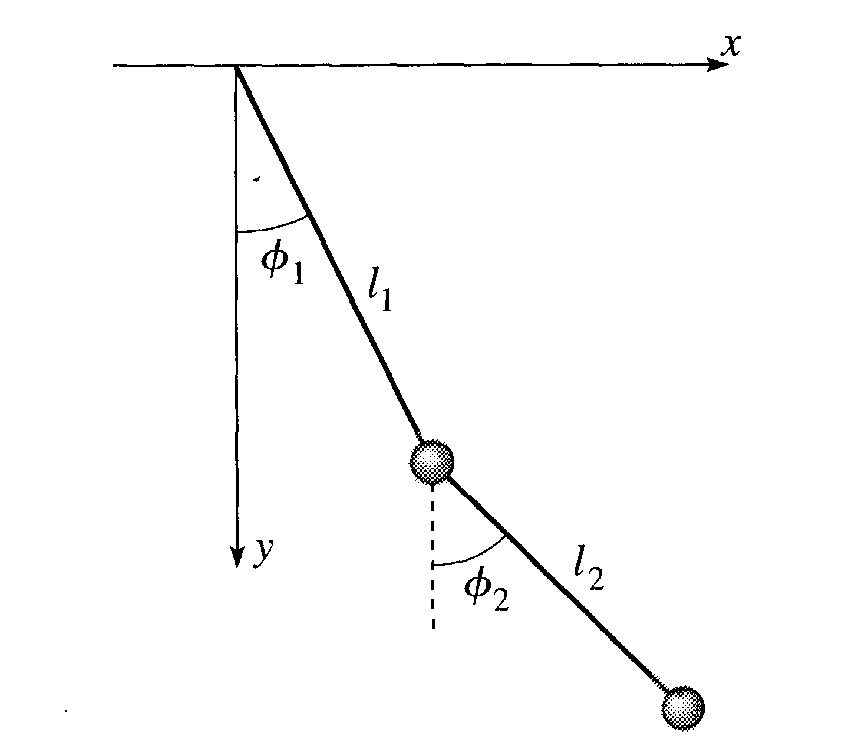
\includegraphics[width=4cm]{doublep.png}
\end{figure}

\subsubsection*{Ex. 3: Transformação dependente do tempo $t$ ($N = 1$ e $n=1$)}

Nos dois exemplos anteriores, as equações de transformação de um sistema para o outro não envolvem o tempo $t$ de forma explícita. Porém, é fácil encontrar exemplos onde isso pode acontecer. Considere a situação onde um pêndulo está preso no teto de um carro e o mesmo se move com aceleração $a$, como ilustra a figura abaixo. Nesse caso, podemos caracterizar completamente o sistema (isto é, especificar a posição da massa presa ao pêndulo) através do ângulo $\phi$. Mas como o carro se move, a relação é dada agora por

\begin{equation}
    \mathbf{r} = (x,y) = (l\sin\phi + \frac{1}{2}at^2,l\cos\phi) = \mathbf{r}(\phi,t),
\end{equation}
onde assumi que em $t = 0$ o ponto de suporte do pêndulo encontrava-se em $x = 0$ com velocidade inicial nula.
\begin{figure}[h]
\centering
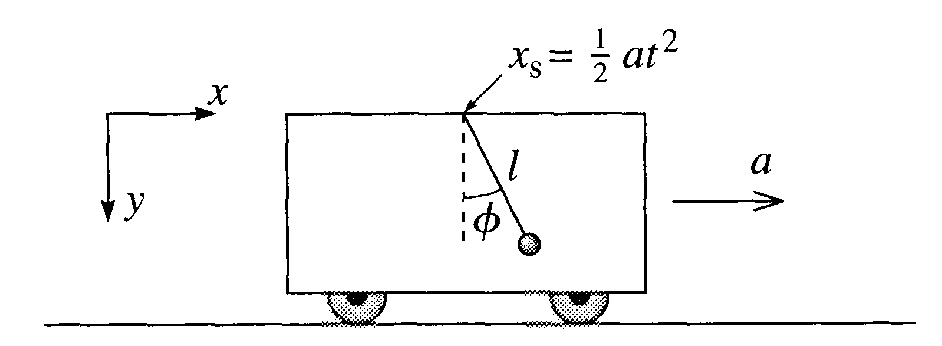
\includegraphics[width=6cm]{car.png}
\end{figure}

Quando a relação entre as coordenadas $\mathbf{r}_\alpha$ e $(q_{1},...,q_n)$ \textbf{não} envolve o tempo $t$, chamamos o conjunto de coordenadas de \textit{natural} \footnote{Algumas vezes ele é chamado de \textit{scleronomous.}}. Felizmente, existe uma grande classe de problemas que se encaixam na categoria de sistemas de coordenadas naturais \footnote{Quando a relação entre as coordenadas envolve o tempo $t$, dizemos que o sistema é \textit{rheonomous}}. Podemos escrever a Lagrangeana do sistema em termos de qualquer sistema de coordenadas generalizadas $(q_1,...,q_n)$. No entanto, como podemos garantir que a Lagrangeana escrita em termos de $(q_1,...,q_n)$ satisfará as mesmas equações de Euler-Lagrange que derivamos na seção anterior utilizando coordenadas cartesianas? Vamos demonstrar esse fato na seção 5. Antes disso, vamos definir os graus de liberdade de um sistema.

\subsection{Graus de Liberdade}

O número de \textit{graus de liberdade} de um sistema é o número de coordenadas que podem ser variadas de maneira independente num pequeno deslocamento - o número de direções ``independentes'' na qual o sistema pode se mover a partir de uma dada configuração inicial. Por exemplo, o pêndulo do Ex. 1 possui um grau de liberdade, enquanto que o pêndulo duplo do Ex. 2 possui dois graus de liberdade. Uma partícula que está livre para se mover no espaço livre possui três graus de liberdade e um gás composto de $N$ partículas possui $3N$.

Quando o número de graus de liberdade de um sistema com $N$ partículas em três dimensões é menor que $3N$, dizemos que o sistema possui um vínculo. (Em duas dimensões, o número correspondente é $2N$ claro) A massa presa ao pêndulo simples possui vínculo, pois $1 < 2N = 2$. O pêndulo duplo também possui vínculo pois $2 < 2N = 4$. Iremos tratar nesta aula apenas os casos onde o número de graus de liberdade do sistema é igual ao número de coordenadas generalizadas. Um sistema com essa propriedade é chamado de holonômico.

\section{Equações de Euler-Lagrange em Coordenadas Generalizadas}

Para simplificar a demonstração, vamos considerar um sistema formado por apenas uma partícula que move-se em apenas uma direção $x$. Nosso objetivo é mostrar que se $L(x,\dot{x})$ satisfaz as Equações de Euler-Lagrange (20), (21) e (22), então $L(q_1,\dot{q_1})$ também satisfarão as mesmas equações onde $q_1$ é a coordenada generalizada. Vamos assumir que $q = q(x)$ e que $x = x(q)$, como foi descrito na seção anterior. Note que $x$ não é função de $\dot{q}$. O Lagrangeano é dado em termos das coordenadas generalizadas por $L = L(q,\dot{q})$. Para começar, tome a derivada parcial de $L(q,\dot{q})$ com relação à $\dot{q}$:
\begin{equation}
\begin{split}
    \frac{\partial L}{\partial \dot{q}} &= \frac{\partial L}{\partial x} \frac{\partial x}{\partial \dot{q}}  + \frac{\partial L}{\partial \dot{x}} \frac{\partial \dot{x}}{\partial \dot{q}} \\
                                        &= \frac{\partial L}{\partial \dot{x}} \frac{\partial \dot{x}}{\partial \dot{q}},
    \end{split}
\end{equation}
pois $x$ não depende de $\dot{q}$. Como $x = x(q)$ podemos escrever
\begin{equation}
    \dot{x} = \frac{\partial x}{\partial q}\dot{q}
\end{equation}
de forma que
\begin{equation}
    \frac{\partial \dot{x}}{\partial \dot{q}} = \frac{\partial x}{\partial q}.
\end{equation}
Substituindo a expressão (25) na equação (23) temos
\begin{equation}
    \frac{\partial L}{\partial \dot{q}} = \frac{\partial L}{\partial \dot{x}}\frac{\partial x}{\partial q}.
\end{equation}
Derivado a equação (26) com relação ao tempo $t$ ficamos com
\begin{equation}
    \begin{split}
        \frac{d}{dt}\frac{\partial L}{\partial \dot{q}} &= \frac{d}{dt}\left( \frac{\partial L}{\partial \dot{x}}\frac{\partial x}{\partial q} \right) \\
                                                        &=\frac{\partial L}{\partial \dot{x}}\frac{d}{dt}\frac{\partial x}{\partial q} + \frac{\partial x}{\partial q}\frac{d}{dt}\frac{\partial L}{\partial \dot{x}} \\
                                                        &= \frac{\partial L}{\partial \dot{x}}\frac{\partial \dot{x}}{\partial q} + \frac{\partial L}{\partial x}\frac{\partial x}{\partial q} \\
                                                        &=\frac{\partial L}{\partial q}.
    \end{split}
\end{equation}
Concluímos então que a equação de Euler-Lagrange satisfeita pelo Lagrangeano $L(q,\dot{q})$ possui a mesma forma matemática das equações escritas com relação ao sistema de coordenadas cartesianas. O resultado pode ser generalizado para qualquer número $N$ de partículas em três dimensões e para qualquer número $M$ de coordenadas generalizadas. A demonstração desse fato fica como exercício para o aluno (ver lista de exercício). 

\section{Forças de Vínculo}

O vínculo existente em um sistema de partículas é o resultado das forças de vínculo. Por exemplo, uma massa no pêndulo está restrita a se mover apenas no arco de circunferência gerado pelo fio, e a força de vínculo é a força que o fio faz na massa. A grande vantagem da formulação Lagrangeana da Mecânica é que não precisamos nos preocupar com as forças de vínculo. Na verdade, em nenhum momento da nossa aula falamos de \textit{força}. Isso se deve ao fato de que o Lagrangeano de uma partícula depende apenas das propriedades da própria partícula (sua energia cinética e potencial). A energia potencial que entrou na função $L$ não inclui as forças de vínculo e, na maioria dos problemas, não estamos interessados em calculá-las, apenas em obter a posição da partícula no decorrer do tempo. É possível demonstrar de maneira mais formal esse resultado (que não farei aqui por ser muito técnico), e para o aluno que deseja um desafio mais rigoroso de matemática, aconselho-o a responder essa questão através da lista de problemas. 

\section{Conclusões} 

\noindent \textbf{CONCLUSÃO GERAL}: Para qualquer sistema holonômico, com $n$ graus de liberdade e $n$ coordenadas generalizadas, e com as forças que não são de vínculos derivadas de uma energia potencial $U(q_1,...,q_n,t)$, o caminho seguido pelo sistema é determinado pelas $n$ equações de Lagrange
\begin{equation}
    \frac{\partial L}{\partial q_i} = \frac{d}{dt}\frac{\partial L}{\partial \dot{q}_i} \hspace{1cm} [i=1,...,n],
\end{equation}
onde $L$ é o Lagrangeano $L = K - U$ e $U = U(q_1,...,q_n,t)$ é a energia potencial total correspondente à todas as forças com exceção das forças de vínculo. 

Note que assumimos que as forças que não são de vínculo são derivadas de uma energia potencial. Se isso não for verdade, então as equações de Lagrange podem não ser satisfeitas, pelo menos na forma da equação (33). Um exemplo óbvio de uma força que não satisfaz essa condição é o atrito. Força de atrito não pode ser vista como uma força de vínculo e não pode ser derivada de uma energia potencial. É possível modificar as equações de Lagrange para incluir o caso de forças dissipativas, mas esse será o assunto de uma outra aula.






\end{document}
